% This file is part of Processorsimulation.
%
% The Processorsimulation is free software: you can redistribute it and/or modify
% it under the terms of the GNU General Public License as published by the Free
% Software Foundation, Version 3.
%
% The Processorsimulation is distributed in the hope that it will be useful, but
% WITHOUT ANY WARRANTY; without even the implied warranty of MERCHANTABILITY or
% FITNESS FOR A PARTICULAR PURPOSE.  See the GNU General Public License for more
% details.
%
% You should have received a copy of the GNU General Public License along with
% this program. If not, see <http://www.gnu.org/licenses/>.

% Author: Eva Charlotte Mayer

\documentclass{article}

\usepackage[ngerman]{babel}
\usepackage{polyglossia}
\setdefaultlanguage{german}
\setotherlanguage[variant=british]{english}
\usepackage{fontspec}
\setmainfont{Latin Modern Roman}

\usepackage[table]{xcolor}
\newcommand{\mc}[2]{\multicolumn{#1}{c}{#2}}
\definecolor{Gray}{gray}{0.85}

\newcolumntype{a}{>{\columncolor{Gray}}c}
\newcolumntype{b}{>{\columncolor{white}}c}

\usepackage{array}
\newcolumntype{L}[1]{>{\raggedright\let\newline\\\arraybackslash\hspace{0pt}}m{#1}}
\newcolumntype{C}[1]{>{\centering\let\newline\\\arraybackslash\hspace{0pt}}m{#1}}
\newcolumntype{R}[1]{>{\raggedleft\let\newline\\\arraybackslash\hspace{0pt}}m{#1}}
\newcolumntype{X}[1]{>{\raggedright\hspace{0pt}}m{#1}}

\usepackage{enumitem}
\setlist{noitemsep}
\setlist[enumerate]{label*=\arabic*.}
\newlist{1enumerate}{enumerate}{5}
\setlist[1enumerate]{label=(\alph*)}
\newlist{2enumerate}{enumerate}{5}
\setlist[2enumerate]{label=(\roman*)}
\newlist{3enumerate}{enumerate}{5}
\setlist[3enumerate]{label=(\Alph*)}
\newlist{5enumerate}{enumerate}{5}
\setlist[5enumerate]{label*=(\arabic*)}

\usepackage[margin=1in, headsep=1cm, headheight=3cm, bottom=1.3in]{geometry}
\addtolength{\topmargin}{0.5in}

\usepackage{tabularx}

\usepackage{graphicx}

\usepackage{fancyhdr}
\pagestyle{fancy}

\usepackage{lipsum}

\usepackage{wrapfig}
\usepackage{subcaption}

\usepackage{listings}

\rhead{
\includegraphics[width=16.5cm, height=1.5cm]{./titel.png}}
\chead{}
\lhead{}
\cfoot{}
\lfoot{ToyProcessor - Version 0.1}
\rfoot{\thepage}
\renewcommand{\footrulewidth}{0.4pt}

\begin{document}

\section*{
\includegraphics[width=1cm]{./icon_umsetzung.png}
\hspace{0.25cm} Was ist ein ToyProcessor?}
Der ToyProcessor ist eine vereinfachte Simulation eines normalen Prozessors in
einem Computer. Die Bauteile des Processors wurden reduziert auf das
Steuerwerk, den RAM (Random-Access-Memory), die ALU (Arithmetic-Logic-Unit),
den Accu (Accumulator), das IR (Instruction register) und den PC (Programm
counter). Der ToyProcessor setzt die Von-Neumann-Architektur um.\\

\noindent \textbf{RAM:}
Im RAM stehen alle Befehle aus dem jeweils geladenen Toy-Programm in binärer oder
hexadezimalen Schreibweise. Der Übersichtlichkeit wegen, sind alle restlichen Einträge
einfach 0 - natürlich entspricht dies nicht dem realistischen Aussehen eines
Speichers. Der RAM kann insgesamt 4096 Einträge beinhalten. Der RAM wird durch das
IR und die ALU ausgelesen und kann durch die ALU auch wieder beschrieben werden.\\

\begin{wrapfigure}{r}{0.7\textwidth}
    \centering 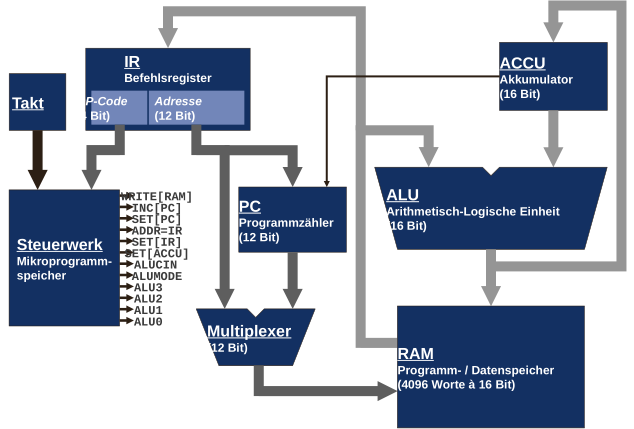
\includegraphics[width=0.65\textwidth]{./picture_processor.png}\\
    \caption*{Abbildung 1: Blockschaltbild des ToyProcessors}
\end{wrapfigure}

\noindent \textbf{ALU:}
In der ALU werden alle Rechenoperationen durchgeführt. Dazu wird der jeweilige
Befehl aus dem RAM und der aktuelle Wert des Akkus geladen und die Operation
ausgeführt. Die ALU kann beim Speicherbefehl den RAM wieder mit dem
Ergebnis beschreiben.\\

\noindent \textbf{Accu:}
Im Accu stehen die aktuellen Werte für eine Rechenoperation zur Verfügung. Diese
werden der ALU zur Verfügung gestellt, wenn sie diese für eine Operation benötigt.
Auch das Ergebnis einer ausgeführten Rechenoperation wird wieder in den Accu geschrieben.
Bei einem Sprungbefehl wird getestet, ob der Accu gleich Null ist.\\

\noindent \textbf{IR:}
Das IR ist das Befehlsregister des Steuerwerks. Hier werden die aktuell zu bearbeitenden
Befehle geladen. Da die Befehle eines Toy-Programms aus 4 Bit OP-Code und 12 Bit Adresse bestehen, kann das
IR ingesamt 16 Bit umfassen.\\

\noindent \textbf{PC:}
Der PC ist zu Anfang eines jeden Toy-Programmes auf Null gesetzt. Nach jedem ausgeführten
Befehl wird er um Eins erhöht. Somit dient er als Indikator, an welcher Stelle sich der
ToyProcessor im Programm im Moment befindet. Er gibt also an, aus welcher Speicherzelle des
RAMs der nächste Befehl ausgelesen werden muss. Bei einem Sprungbefehl wird der PC auf
den Wert gesetzt, zu dem gesprungen werden soll.\\

\noindent \textbf{Steuerwerk:}
Das Steuerwerk führt die jeweiligen Befehle aus, die es aus dem IR übergeben bekommt.
Da die Befehle eines Toy-Programms aus verschiedenen Teilbefehlen bestehen (siehe "Wie
läuft ein Toy-Programm ab?") leuchten in jedem Takt die Flags zu den zugehörigen Teilbefehlen
auf, die aktuell durchgeführt werden. Diese sind links des Steuerwerkblocks zu erkennen. \\

\newpage

\section*{
\includegraphics[width=1cm]{./icon_ablauf.png}
\hspace{0.25cm} Wie läuft ein Toy-Programm ab?}
Der ToyProcessor kann 12 Befehle verarbeiten. Intern hat ein Befehl immer das folgende Format: Die erste 4 Bit entsprechen
dem OP-Code, welcher die jeweils auszuführende Operation spezifiziert. Die
letzten 12 Bit geben die Adresse an, an der der Wert im RAM liegt, mit dem
die jeweilige Operation durchgeführt werden soll. Das Ergebnis einer Operation
wird immer in den Accu geschrieben. Die Steuerung der auszuführenden
Befehle erfolgt im 2-Phasen-Takt:

\begin{figure}[h!]
    \centering
    \begin{minipage}{0.49\textwidth}
        \centering
        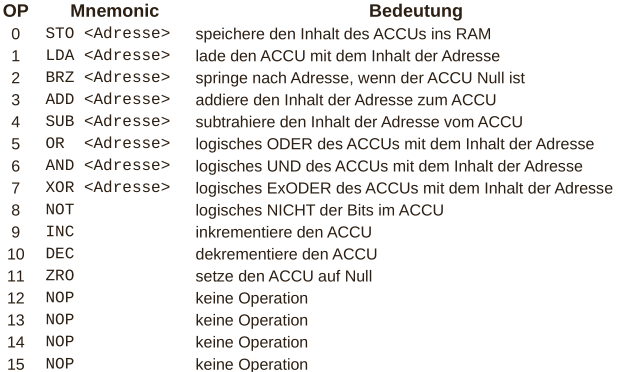
\includegraphics[height=0.6\linewidth]{./picture_befehlssatz.png}
        \caption*{Abbildung 2: Befehlssatz des ToyProcessors}
    \end{minipage}
    \begin{minipage}{0.49\textwidth}
        \centering
        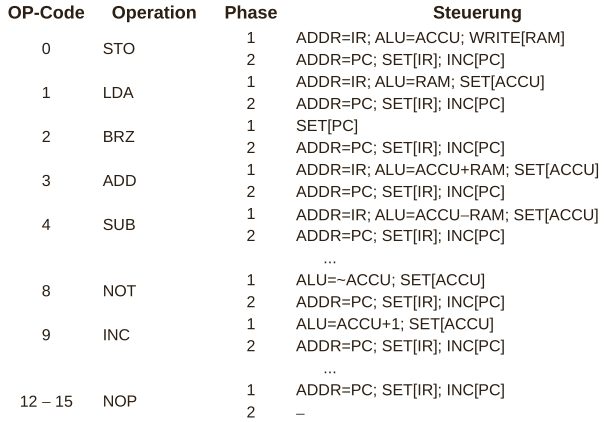
\includegraphics[height=0.6\linewidth]{./picture_steuerung.png}
        \caption*{Abbildung 3: Steuerung der Toy-Befehle}
    \end{minipage}
\end{figure}

\section*{
\includegraphics[width=0.95cm]{./icon_stift.png}
\hspace{0.25cm} Wie schreibe ich ein Toy-Programm?}

\begin{wrapfigure}{r}{9cm}
\centering
\begin{tabular}{|p{3cm}|p{3cm}|p{3cm}|}
    \hline
    & & \\
    \textbf{Binär:} & \textbf{Hexadezimal:} & \textbf{Assembler}\\
    & & \\
    \hline
    0000xxxxxxxxxxxx & \$0yyy & STO z \\
    0001xxxxxxxxxxxx & \$1yyy & LDA z \\
    0010xxxxxxxxxxxx & \$2yyy & BRZ z \\
    0011xxxxxxxxxxxx & \$3yyy & ADD z \\
    0100xxxxxxxxxxxx & \$4yyy & SUB z \\
    0101xxxxxxxxxxxx & \$5yyy & OR z \\
    0110xxxxxxxxxxxx & \$6yyy & AND z \\
    0111xxxxxxxxxxxx & \$7yyy & XOR z \\
    1000xxxxxxxxxxxx & \$8yyy & NOT \\
    1001xxxxxxxxxxxx & \$9yyy & INC \\
    1010xxxxxxxxxxxx & \$Ayyy & DEC \\
    1011xxxxxxxxxxxx & \$Byyy & ZRO \\
    1100xxxxxxxxxxxx & \$Cyyy & NOP \\
    1101xxxxxxxxxxxx & \$Dyyy & NOP \\
    1110xxxxxxxxxxxx & \$Eyyy & NOP \\
    1111xxxxxxxxxxxx & \$Fyyy & NOP\\
    \hline
\end{tabular}
\centering \caption*{Tabelle 1: Binär-, Hexadezimal- und Assemblerdarstellung der Toy-Befehle}
\end{wrapfigure}
\hspace{20cm}\\Es gibt vier unterschiedliche Möglichkeiten ein Toy-Programm zu schreiben:
Die Befehle können sowohl in binärer und in hexadezimaler Schreibweise, als
auch in Assembler (= Mnemonic, vgl. Abbildung 2) kodiert werden. Außerdem gibt es noch die Möglichkeit
Pseudo-C-Code zu verfassen. \\\\Die Tabelle rechts umfasst die Binär-,\\ Hexadezimal-
und Assemblervarianten. Die "xxxxxxxxxxxx" kodieren die Adresse für den
jeweiligen OP-Code in binär, "yyy" stehen für die Adresse in hexadezimal und
"z" gibt die Adresse als Dezimalzahl an.\\\\ Wir werden nun das Programmieren mit den
Toy-Befehlen an einigen Beispielen üben. Am Ende dieses Absatzes werden wir dann noch auf die
Einschränkungen des Pseudo-C-Codes eingehen.\\\\\\

\noindent \large \underline{\textbf{Binär-, Hexadezimal- und Assemblerprogrammierung}}\\

\normalsize
\noindent \textbf{Format:} Das Toy-Programm sollte in einem simplen Texteditor geschrieben werden. Die Textdatei
sollte die Endung *.toy bekommen.\\

\noindent \textbf{Code:} Die einzelnen Befehle werden alle untereinander in jeweils neue Zeilen geschrieben.
In den RAM werden sie in der gleichen Reihenfolge geschrieben, angefangen bei
der nullten Speicherzelle.
Wie man der Tabelle 1 entnehmen kann, sind die verschiedenen Varianten (binär, hexadezimal und
Assembler) äquivalent, daher können diese im Source-Code gemischt werden. Beispielsweise
liefern somit die folgenden drei Toy-Programme zum Subtrahieren der Werte aus RAM[11] und RAM[22]
dasselbe Ergebnis:
\begin{figure}[h!]
    \centering
    \begin{subfigure}[b]{0.45\textwidth}
\begin{lstlisting}
0001000000001011
0100000000010110
0000000000001011
\end{lstlisting}
        \caption{Binär}
   \end{subfigure}
   \begin{subfigure}[b]{0.15\textwidth}
\begin{lstlisting}
$100B
$4016
$000B
\end{lstlisting}
        \caption{Hexadezimal}
    \end{subfigure}
    \begin{subfigure}[b]{0.15\textwidth}
\begin{lstlisting}
LDA 11
SUB 22
STO 11
\end{lstlisting}
        \caption{Assembler}
    \end{subfigure}
    \begin{subfigure}[b]{0.2\textwidth}
\begin{lstlisting}
0001000000001011
$4016
STO 11
\end{lstlisting}
        \caption{Gemischt}
    \end{subfigure}
\end{figure}

\noindent \textbf{RAM-Settings:} Um mit konkreten Werten zu rechnen, können diese direkt in den RAM geschrieben
und die RAM-Adresse für die jeweiligen Rechenoperationen benutzt
werden. Angenommen, wir würden bei unserem Beispiel gerne 42 von 84 abziehen,
so sähe das ganze wie in der folgenden Tabelle aus: Die ersten zwei Zeilen des jeweiligen
Programms setzen RAM[11]=84 und RAM[22]=42, das Ergebnis wird wie oben in
RAM[11] gespeichert. Die einzige Einschränkung bezüglich RAM-Setting ist, dass Werte nur in
Speicherzellen geschrieben werden dürfen, welche eine höhere Nummer als die Anzahl an OP-Codes im
Toy-Programm haben. Es wäre hier also nicht erlaubt gewesen, die Speicherzellen
0, 1 oder 2 zu beschreiben, da das Toy-Programm insgesamt 3 OP-Codes beinhaltet. Achtung: Binäre Ramsettings,
die kürzer als 16 Bit sind, werden als Dezimalzahlen interpretiert.
\begin{figure}[h!]
    \centering
    \begin{subfigure}[b]{0.45\textwidth}
\begin{lstlisting}
:0000000000001011:0000000001010100
:0000000000010110:0000000000101010
0001000000001011
0100000000010110
0000000000001011
\end{lstlisting}
        \caption{Binär}
   \end{subfigure}
   \begin{subfigure}[b]{0.15\textwidth}
\begin{lstlisting}
:$00B:$054
:$016:02A
$100B
$4016
$000B
\end{lstlisting}
        \caption{Hexadezimal}
    \end{subfigure}
    \begin{subfigure}[b]{0.15\textwidth}
\begin{lstlisting}
:11:84
:22:42
LDA 11
SUB 22
STO 11
\end{lstlisting}
        \caption{Assembler}
    \end{subfigure}
    \begin{subfigure}[b]{0.2\textwidth}
\begin{lstlisting}
:$00B:$054
:22:42
0001000000001011
$4016
STO 11
\end{lstlisting}
        \caption{Gemischt}
\end{subfigure}
\end{figure}

\noindent \textbf{Endlosschleife:} Um zu verdeutlichen, dass ein Prozessor
niemals aufhört zu arbeiten, muss jedes Toy-Programm in einer Endlosschleife
enden. Dies kann durch das Hinzufügen eines "ZRO" (= Setze den Accu auf Null)
und eines "BRZ <einen Befehl davor>" (= Springe zum Befehl davor, d.h. zu ZRO,
falls der Accu Null ist) am Ende des Toy-Programms erreicht werden.
\begin{figure}[h!]
    \centering
    \begin{subfigure}[b]{0.45\textwidth}
\begin{lstlisting}
:0000000000001011:0000000001010100
:0000000000010110:0000000000101010
0001000000001011
0100000000010110
0000000000001011
1011000000000000
0010000000000011
\end{lstlisting}
        \caption{Binär}
   \end{subfigure}
   \begin{subfigure}[b]{0.15\textwidth}
\begin{lstlisting}
:$00B:$054
:$016:02A
$100B
$4016
$000B
$B000
$2003
\end{lstlisting}
        \caption{Hexadezimal}
    \end{subfigure}
    \begin{subfigure}[b]{0.15\textwidth}
\begin{lstlisting}
:11:84
:22:42
LDA 11
SUB 22
STO 11
ZRO
BRZ 3
\end{lstlisting}
        \caption{Assembler}
    \end{subfigure}
    \begin{subfigure}[b]{0.2\textwidth}
\begin{lstlisting}
:$00B:$054
:22:42
0001000000001011
$4016
STO 11
1011000000000000
$2003
\end{lstlisting}
        \caption{Gemischt}
\end{subfigure}
\end{figure}

\newpage

\noindent \textbf{Kommentare:}
Kommentare können mit "\#" gesetzt werden. Wir kommentieren hier nun zur
Veranschaulichung die Assembler-Variante unteres Toy-Programms - für die
anderen Varianten funktioniert das Kommentieren analog:
\begin{figure}[h!]
\begin{lstlisting}
#RAM-Settings
:11:84  #RAM[11] wird auf den Wert 84 gesetzt
:22:42  #RAM[22] wird auf den Wert 42 gesetzt

#Subtraktion der beiden Werte
LDA 11  #Läd 84, den Wert aus RAM[11]
SUB 22  #Subtrahiert davon 42, den Wert aus RAM[22]
STO 11  #Speichert das Ergebnis in RAM[11]

#Endlosschleife
ZRO     #Setzt den Accu auf Null
BRZ 3   #Springt zurück zum ZRO Befehl in RAM[3]
\end{lstlisting}
\end{figure}

\normalsize

\noindent \textbf{Variablen:} Im Assemblercode können anstatt RAM-Settings
auch Variablen deklariert werden. Diese werden dann vom ToyProcessor automatisch
in Speicherzellen nach den OP-Codes geschrieben. Variablen werden wie folgt
deklariert: "<variablenname> = <wert>".
Variablennamen dürfen aus Groß- und Kleinbuchstaben, sowie Zahlen bestehen.
Die zugewiesenen Werte dürfen eine Dezimal- oder Hexadezimalzahl sein.
Es dürfen keine RAM-Settings und Variablendeklarationen gleichzeitig in einem Toy-Programm
vorkommen. Des weiteren kann der Assembler mit Variablen und später auch Labeln
nicht mehr mit binärem oder hexadezimalem Code gemischt werden.
Hier das obige Beispiel mit Variablendeklarationen anstatt den RAM-Settings:
\begin{figure}[h!]
\begin{lstlisting}
#Variablendeklarationen
a = 84  #Deklariere eine Variable mit dem Namen a und dem Wert 84
b = $2A  #Deklariere eine Variable mit dem Namen b und dem Wert 0x2A = 42

#Subtraktion der beiden Variablenwerte
LDA a  #Läd die Variable a mit dem Wert 84
SUB b  #Subtrahiert davon die Variable b mit dem Wert 42
STO a  #Speichert das Ergebnis in Variable a

#Endlosschleife
ZRO     #Setzt den Accu auf Null
BRZ 3   #Springt zurück zum ZRO Befehl in RAM[3]
\end{lstlisting}
\end{figure}

\noindent \textbf{Labels:} Labels dienen als Anhaltspunkte, wohin ein
Sprungbefehl im Code zurückkehren muss. Labels können also anstatt der
RAM-Adresse des Befehls, zu dem zurückgesprungen werden soll, angegeben werden.
Labels werden im Stil von: "<labelname>:"
deklariert. Labelnamen dürfen Groß- und Kleinbuchstaben, aber keine Zahlen
enthalten. Unsere Endlosschleife könnten wir mit Hilfe von Labels also
wie folgt gestalten:
\begin{figure}[h!]
\begin{lstlisting}
#Endlosschleife
loop:
ZRO         #Setzt den Accu auf Null
BRZ loop    #Springt zurück zum ZRO Befehl, da dieser nach dem Label "loop" kommt
\end{lstlisting}
\end{figure}

\newpage
\vspace{-5cm}
\noindent \large \underline{\textbf{Pseudo-C-Code}}\\

\normalsize
\noindent \textbf{Datentypen:} Da dem ToyProcessor nur 16 Bit lange Befehle zur
Verfügung stehen, dürfen nur die Datentypen "short int", "char" und "bool"
benutzt werden. Selbstverständlich dürfen diese ihren Wertebereich nicht
überschreiten. Chars können außerdem nur Zahlen und keine Buchstaben zugewiesen
werden. \\

\noindent \textbf{Rechenoperationen:} Es sind alle Rechenoperationen, die
auch der ToyProcessor durchführen kann, erlaubt. Das heißt:
+, -, |, \&, \^, !, ++, - - .
Zu beachten hierbei ist, dass die Operanden einer Rechenoperation immer
an Variablen gebunden sein müssen und nicht beliebige Zahlenwerte sein können.
Somit wären die Statements links erlaubt und die Statements rechts nicht: (Angenommen,
dass die Variablen a und c richtig deklariert wurden.)
\begin{lstlisting}
    a = a + b;                      a = a + 4;  # nicht erlaubt
    c = !c;                         c = 1 | 0;  # nicht erlaubt
\end{lstlisting}

\noindent Außerdem können keine Klammern verwendet werden und nicht mehrere Operationen in einer
Reihe durchgeführt werden. Sollen also mehrere Rechenoperationen
auf einer Variablen gemacht werden, müssen diese in ihre Teilschritte heruntergebrochen werden.
Beispielsweise müsste der Ausdruck links, wie folgt umgewandelt werden (siehe rechts, nach jedem Semicolon
soll dort jeweils eine neue Zeile angefangen werden.):
\begin{lstlisting}
    a = b | (c - d + e);    --->    a = c - d; a = a + e; a = b | a
\end{lstlisting}

\noindent \textbf{Konstrukte:}
\begin{itemize}
    \item   If-Statements werden analog zum normalen
            C-Code deklariert. Jedoch können If-Statements in Toy-Programmen nur darauf testen, ob
            Variablen ungleich Null sind, d.h. if(var != 0) oder if(var).
    \item   While-Schleifen werden genau so, wie in
            normalem C deklariert. Die Abbruchkonditionen im Pseudo-C-Code darf jedoch
            nur darauf testen, ob eine Variable ungleich null ist.
    \item   For-Schleifen werden auch analog zum
            bekannten C-Code geschrieben. Die Laufindexvariablen werden grundsätzlich in der
            for-Schleife selbst deklariert. Es sind jedoch nur folgende Konstruktionen
            erlaubt (sei "i" eine undeklarierte Variable, "x" und "y" beliebige
            Dezimalwerte):\\
            for(short int i = x; i < y; i++) bzw. for(short int i = x; i > y; i++) bzw.
            for(short int i = x; i < y; i- -) und for(short int i = x; i > y; i- -)
\end{itemize}

\noindent \textbf{Weiteres:}
Im Pseudo-C-Code wird keine Endlosschleife am Ende des Toy-Programmes benötigt,
da diese automatisch vom ToyProcessor hinzugefügt wird. Außer den oben
beschriebenen C-Konstrukten sind alle anderen Datentypen, Operationen,
Funktionen, Library-Elemente etc. nicht erlaubt. Kommentare funktionieren
genauso, wie bei der Binär-, Hexadezimal- und Assemblerprogrammierung. Beispiel eines Pseudo-C-Code-Toy-Programm:
\begin{lstlisting}
    short int a = 0;
    char b = 10;
    bool c = 1;

    if (c) {
        #Schleife, die a = 10 + 9 + 8 + ... + 1 = 55 rechnet.
        while (b != 0) {
            a = a + b;
            #Schleife, die nur als Demonstration von for-Loops dient.
            for(short int i = 4; i < 6; i++) {
                a++;
                a--;
            }
            b--;
        }
    }
\end{lstlisting}

\section*{
\includegraphics[width=1cm]{./icon_bedienung.png}
\hspace{0.25cm} Bedienung}

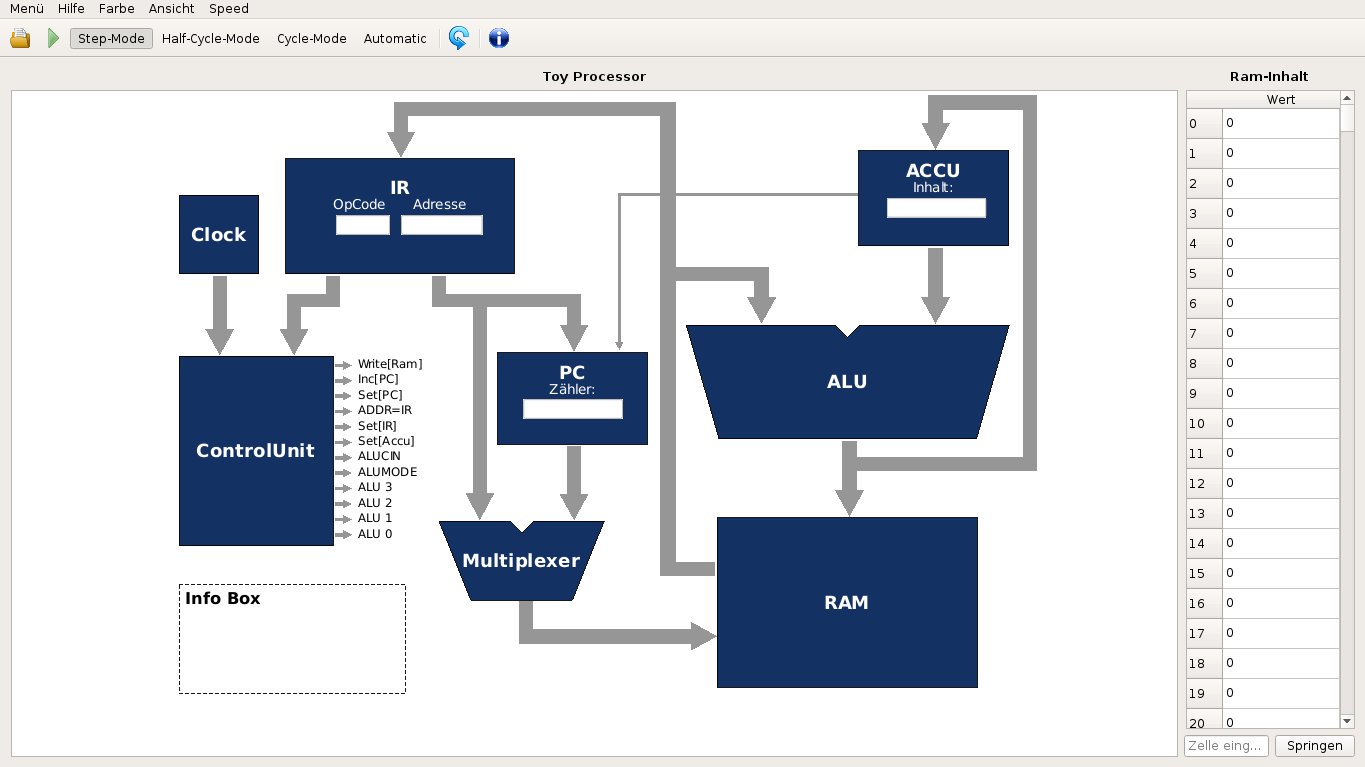
\includegraphics[width=\textwidth]{./picture_gui.png}\\\\
\noindent Das Bild oben zeigt die GUI des ToyProcessors an. In der Mitte ist das Blockschaltbild des ToyProcessors erkennbar. Die Pfeile zwischen den
einzelnen Prozessoreinheiten sind noch grau, sie werden erst beim Ausführen eines Programms (genau gesagt
beim Ausführen eines Befehls) gefärbt. Die Einzelteile werden wie folgt bedient:\\

\noindent \textbf{Steuerungsleiste:} In der Steuerungsleiste ganz oben befinden sich 8 verschiedene
Buttons/Optionen:
\begin{itemize}
    \item   Mit dem Button ganz rechts kann ein Programm in den ToyProcessor geladen werden.
    \item   Der grüne Pfeil daneben dient zum Starten des AutomaticModus bzw. zum Durchklicken in den anderen Modi.
    \item   Mit der Auswahl eines der vier Buttons "Step-Mode", "Half-Cycle-Mode" und "Cycle-Mode" kann festgelegt werden, wieviele
            der Einzelschritte eines Befehles (siehe Abbildung 3) gleichzeitig ausgeführt werden.
    \item   Ist "Automatic" gewählt, dann werden die Befehle nacheinander abgearbeitet, bis das Programm in die Endlosschleife gerät.
    \item   Der Button mit dem gekringelten blauen Pfeil setzt das Programm zurück auf den Anfang des geladenen Programms.
    \item   Durch das Klicken des Buttons ganz rechts kann man die Dokumentation ansehen.
\end{itemize}

\noindent \textbf{Direktes Manipulieren von Werten:}
In das Instruction Register (IR), den Programmcounter (PC) und den Accu können direkt Werte geschrieben werden. Dazu dienen die Textfelder in den jeweiligen Bausteinen.  Dies ermöglicht es, dass Programm
während der Laufzeit zu verändern, indem z.B. durch das Umschreiben des PC-Wertes an eine andere Stelle gesprungen oder im Instruction Register ein
neuer Befehl ausgeführt wird. Am Anfang stehen die Werte alle auf Null. Fehlerhafte Eingaben werden abgefangen.\\

\newpage

\begin{wrapfigure}{r}{0.45\textwidth}
    \centering 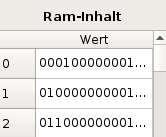
\includegraphics[width=0.2\textwidth]{./picture_ramBinary.png}\\
    \vspace{.1cm}
    \centering 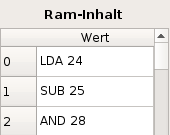
\includegraphics[width=0.2\textwidth]{./picture_ramAssembly.png}\\
    \caption*{Abbildung 4: Binär- und Mnemonicdarstellung des RAMs}
\end{wrapfigure}
\noindent \textbf{RAM-Anzeige:}
Ganz rechts wird der Inhalt des RAMs in einer Tabelle angezeigt. Ist noch kein Programm geladen, so sind alle Einträge Null - dies entspricht natürlich nicht der
Realität, in der die unterschiedlichsten Werte im Speicher stehen können, bis sie überschrieben werden. Sobald ein Toy-Programm geöffnet wurde, erscheinen die
Werte in der Tabelle und das Programm kann ausgeführt werden. Der aktuell ausgeführte Befehl wird grau unterlegt. Alle Werte im RAM können sowohl als Dezimalzahlen,
als auch Hexadezimalzahlen dargestellt werden. Umgestellt wird dies im Menü "Ansicht --> Darstellung".\\\\\\

\noindent \textbf{Weitere Einstellungen:}
\begin{itemize}
    \item   Unter "Farbe" können die Farben für aktive und inaktive Pfeile beliebig gewählt werden. Als Beispiel siehe die Abbildungen unten.
    \item   Unter "Ansicht" kann entschieden werden, ob die exakten Pfade, die genau zeigen, welche Bausteine in einem Schritt angesprochen werden, oder die
            ganzen Pfade, die der Realität entsprechen, angezeigt werden. Außerdem kann im Unterpunkt die Werteanzeige in den Bausteinen zwischen den Formaten dezimal, binär,
            hexadezimal und mnemonic verändert werden.
    \item   Unter "Speed" kann die Schnelligkeit des AutomatikModus gesetzt werden.
\end{itemize}

\vspace{1cm}

\begin{figure}[h!]
    \centering
    \begin{minipage}{0.49\textwidth}
        \centering
        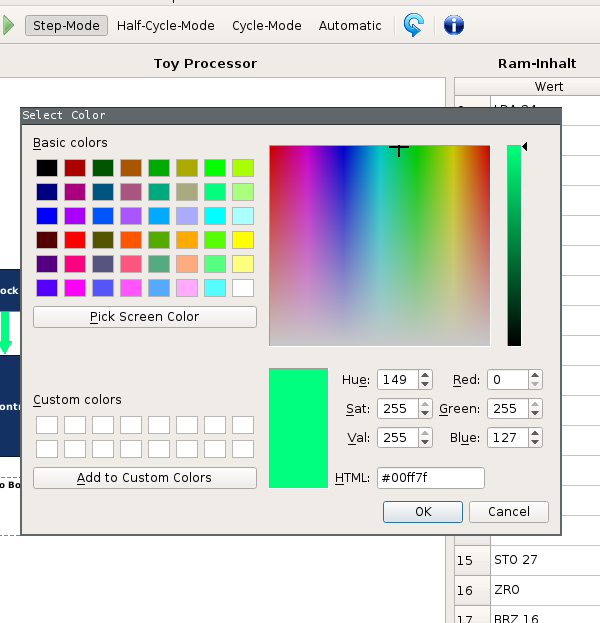
\includegraphics[height=0.6\linewidth]{./picture_farbauswahl.png}
        \caption* {Abbildung 5: Auswahl der Farbe für die Pfeile}
    \end{minipage}
    \begin{minipage}{0.49\textwidth}
        \centering
        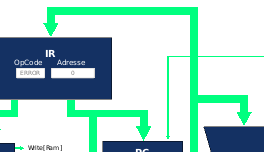
\includegraphics[height=0.6\linewidth]{./picture_pfeile.png}
        \caption*{Abbildung 6: Veränderte Pfeile}
    \end{minipage}
\end{figure}

\vspace{1cm}

\noindent \textbf{Menükürzel:}\\\\
\noindent \begin{tabular}{lllllll}
    Datei laden & Strg+Umschalt+E & & & & Half-Cycle-Mode & Strg+2\\
    Beenden & Strg+Umschalt+Q & & & & Cycle-Mode & Strg+3\\
    Dokumentation & Strg+I & & & & Automatic & Strg+4\\
    Start/Next Step & Leertaste & & & & Reset & Strg+R\\
    Step-Mode & Strg+1 & & & & &
\end{tabular}

\newpage

\section*{
\includegraphics[width=1cm]{./icon_literatur.png}
\hspace{0.25cm} Literaturverzeichnis}
\begin{enumerate}
    \item   Prof. Dr. Bringmann, Foliensatz 7 "Register Transfer Ebene" der Vorlesung "Einführung
            in die technische Informatik", 13.11.2013
    \item   Phil Koopman, "Microcoded versus hard-wired control", BYTE,
            Januar 1987, S. 235, (vgl. www.ece.cmu.edu/~koopman/ - Zugriff am
            15.06.2015)
    \item   Fiete Botschen, "Toy Processor - Beta 0.4 Documentation",
            17.10.2014
    \item   https://en.wikipedia.org/wiki/Instruction\_register - Zugriff
            am 14.06.2015
    \item   www.whatis.techtarget.com/definition/program-counter - Zugriff
            am 14.06.2015
\end{enumerate}

\end{document}
